\chapter{Development of the chosen solutions}

Once we have defined what we want to do in the previous chapter, \textbf{Methodology, Considerations, and Decisions on Alternative Solutions}, it is time to get to work.

\section{Graphic interface [DONE]}

One important point is to provide a GUI (\textit{Graphical User Interface}) that is intuitive and easy to use. Since Python is being used for development, the chosen solution is to use the Tkinter\cite{Tkinter} library for the window and page system, and the Matplotlib\cite{Matplotlib} library to display graphical results of certain analysis algorithms.

As Tkinter works, all actions that need to be triggered or modified through user interaction must be handled inside a function. Therefore, the way this library operates is by calling predefined functions in response to any user interaction.

First, we need to define the graphical architecture, where each module will be integrated into the graphical user interface. Since the program functions as a set of tools, we must define where each tool will be placed within the interface.

These tools can be divided into two important groups, which will also correspond to two separate windows accessible from the root window:

\begin{itemize}
	\item \textbf{Analysis Window:} This window will contain the tools that need to receive sound from both the external input and the system input (Input from System). It will then display the results of the analysis performed on those signals.
	\item \textbf{DSP Window:} This window, also called the \textbf{"Correction Window"}, contains the tools that receive sound from the external input, as well as data indicating how the signal should be processed, and then send the processed signal to the output (Output to System).
\end{itemize}

Each of these two windows will be divided into pages, with each page containing a specific tool. Additionally, a settings window is needed, where the user can set global parameters. With all of this, we arrive at the following GUI scheme:

\begin{figure}[H]
	\begin{center}
		\vspace{-2mm}
		\tikzsetnextfilename{GUI_path}
		\begin{tikzpicture}[node distance=30mm,on grid,auto, scale=1, bend angle=45]
			
			every node/.style={font=\small};
			
			\node (q_root) [draw, rectangle, minimum size=1cm] {ROOT WINDOW};
			%\node (null_ext) [right=of q_ext] {};
			\node (q_ana) [draw, rectangle, minimum size=1cm, xshift=-3cm, below left=of q_root]{ANALYSIS WINDOW};
			\node (q_dsp) [draw, rectangle, minimum size=1cm, xshift=3cm, below right=of q_root]{DSP WINDOW};
			\node (q_set) [draw, rectangle, minimum size=1cm, yshift=1cm, below=of q_root]{SETTINGS WINDOW};
			\node (q_dev) [draw, rectangle, minimum size=1cm, xshift=2cm, yshift=1cm, below=of q_set]{Device Settings Page};
			\node (q_aud) [draw, rectangle, minimum size=1cm, xshift=-2cm, yshift=1cm, below=of q_set]{Audio Settings Page};
			\node (q_eq) [draw, rectangle, minimum size=1cm, yshift=-1cm, below=of q_dsp]{EQ Page};
			\node (q_ft) [draw, rectangle, minimum size=1cm, yshift=-3cm, below left=of q_ana]{FT Page};
			\node (q_31) [draw, rectangle, minimum size=1cm, right=of q_ft]{31 Bands Page};
			\node (q_del) [draw, rectangle, minimum size=1cm, right=of q_31]{Delay Page};
			
			\draw[blue, very thick, ->] (q_root) edge node {} (q_ana);
			\draw[blue, very thick, ->] (q_root) edge node {} (q_set);
			\draw[blue, very thick, ->] (q_root) edge node {} (q_dsp);
			\draw[green, very thick, ->] (q_dsp) edge node {} (q_eq);
			\draw[green, very thick, ->] (q_set) edge node {} (q_aud);
			\draw[green, very thick, ->] (q_set) edge node {} (q_dev);
			\draw[green, very thick, ->] (q_ana) edge [bend right=10] node {} (q_ft);
			\draw[green, very thick, ->] (q_ana) edge [bend right=12.5] node {} (q_31);
			\draw[green, very thick, ->] (q_ana) edge [bend right=15] node {} (q_del);

			
		\end{tikzpicture}
		\vspace{-2mm}
	\end{center}
	\caption{GUI window schematic}
\end{figure}

To make coding a bit easier, I will take advantage of the different pages to split the code across multiple Python files. In total, there are five files:

\begin{itemize}
	\item \textbf{rta+c.py:} This is the root file that contains all initial instructions and the root window. It is the file that must be executed to start the program. Its name stands for \textbf{Real Time Analysis plus Correction}, which is also the name of the program.
	\item \textbf{settings.py:} This file contains the settings window and its associated pages.
	\item \textbf{dsp.py:} This file contains the DSP (correction) window.
	\item \textbf{analysis.py:} This file contains the analysis window and all its pages.
	\item \textbf{config.py:} This file declares some important variables that must be accessible from anywhere in the program. It does not contain any GUI-related elements.
\end{itemize}

Since the GUI layer is responsible for executing most of the program’s modules, each window’s file also contains all the necessary functions for analysis, processing, and plotting. In addition, all pages follow, as much as possible, the same structure in order to maintain the program’s logic and readability. This structure is based on three parts:

\begin{enumerate}
	\item \textbf{Initialize:} This section initializes the objects needed, sets up the plots with empty data, and defines the labels that will be displayed on the page.
	\item \textbf{Update:} A function that contains the analysis algorithms, draws data on the plots, or runs DSP algorithms. This update function is called in every iteration of the algorithm loop using Tkinter methods.
	\item \textbf{Control:} This final part contains the control parameters, flags, and buttons that affect the update function.
\end{enumerate}

One very important aspect of using Tkinter is object management. By default, common Python classes may not work properly under certain GUI rendering conditions. To avoid this, when an object needs to be accessible from any page of the GUI, I use three different solutions: use of \textit{config.py} as a shared configuration module containing predefined objects, which can be accessed from anywhere by importing this file; use of \textit{global} and \textit{nonlocal} objects inside the same window; and use of Tkinter classes such as \textit{tkinter.IntVar}.

Finally, even though Tkinter offers a default way to close windows using the "X" symbol in the top left corner of the window, it does not always work properly—it may simply erase the window but not stop the process that is running from that window. To correctly close any window, it is important to define a close function. This function will be executed when the user clicks the "X" symbol, replacing the default function.

\begin{minted}[label=\texttt{ipython}]{python3}
	"""
	In this case, this is the function that closes the root window and, as a consequence, the entire program.
	"""
	
	# Close all
	def on_close_all():
		config.update_enabled = False # Prevent all periodic updates
		stop_global_stream()  # Ensure the stream is stopped
	
		time.sleep(0.5)
		root.destroy()
	
	root.protocol("WM_DELETE_WINDOW", on_close_all)
	
\end{minted}



\section{Signal Path [DONE]}

To perform any kind of analysis or signal processing, the first thing we need is data—more specifically, signal data captured from the sound card. This data is sent to different modules so that each one can carry out its specific task. Additionally, in the case of the correction module, it is necessary to send output data back to the sound card (the corrected signal). Additionally, there will be non-signal data containing the results of the analysis, which will be sent to the DSP (\textit{Digital Signal Processor}) or the correction window.

\begin{figure}[H]
	\begin{center}
		\vspace{-2mm}
		\tikzsetnextfilename{general_path}
		\begin{tikzpicture}[node distance=30mm,on grid,auto, scale=1, bend angle=45]
			
			every node/.style={font=\small};
			
			\node (q_ext) {External Input};
			\node (null_ext) [right=of q_ext] {};
			\node (q_ana) [draw, rectangle, minimum size=1cm, below right=of null_ext]{Analysis Window};
			\node (q_dsp) [draw, rectangle, minimum size=1cm, above right=of null_ext]{DSP Window};
			\node (q_out) [right=of q_dsp, xshift=2cm]{Output to System};
			\node (q_inp) [right=of q_ana, xshift=2cm]{Input form System};
			
			
			%\node (q_delay) [draw, rectangle, minimum size=1cm, right=of null_init] {Delay Buffer};
			%\node (q_ext) [draw, rectangle, minimum size=1cm, above right=of q_delay, xshift=2cm] {Filtering and RMS Calculation of External Input};
			%\node (q_in_sys) [draw, rectangle, minimum size=1cm, below right=of q_delay, xshift=2cm] {Filtering and RMS Calculation of Input from System};
			%\node (q_diff) [draw, rectangle, minimum size=1cm, right=of q_delay, xshift=4cm] {Difference calculation};	
			
			\draw[blue, very thick, ->] (q_ext) edge node {} (q_ana);
			\draw[blue, very thick, ->] (q_ext) edge node {} (q_dsp);
			\draw[blue, very thick, ->] (q_dsp) edge node {} (q_out);
			\draw[blue, very thick, ->] (q_inp) edge node {} (q_ana);
			\draw[green, dotted, very thick, ->] (q_ana) edge [bend right=10] node {Data} (q_dsp);
			%\draw[blue, dotted, very thick, ->] (q_delay) edge[bend right=10] node {1 channel} (q_ext);
			%\draw[blue, dotted, very thick, ->] (q_delay) edge[bend right=10] node {1 channel} (q_in_sys);
			%\draw[green, very thick, ->] (q_ext) edge[bend right=10] node {Analysis Data} (q_diff);
			%\draw[green, very thick, ->] (q_in_sys) edge[bend right=10] node {Analysis Data} (q_diff);
			
		\end{tikzpicture}
		\vspace{-2mm}
	\end{center}
	\caption{Basic representation of the required signal path}
\end{figure}

To achieve real-time processing, we must manage a constant flow of data. For this purpose, I will use a stream-style data management approach, which consists of capturing small blocks of data, processing them, and continuously sending the results. To capture and send this stream to and from the sound card, the Sounddevice library \cite{sounddevice} will be used.

To simplify things, the two required inputs—\textbf{External Input} and \textbf{Input from System}—will be handled using a single input stream, while the output—\textbf{Output to System}—will be managed through a separate, independent output stream. All streams will share the same parameters, such as bit depth, sample rate, and block size. However, the audio device and channel parameters will be independently set for each stream. In the case of the input stream, each input channel must also be configured separately.

Once the streams are running and managed from the root window, we need to handle the data coming from the input streams and the data to be sent to the output stream. To achieve this, I will use one input buffer for both input channels and a separate output buffer. These buffers must be accessible to all tool modules in the program and will be locked whenever a module accesses them, in order to prevent simultaneous reads and writes.

\begin{figure}[H]
	\begin{center}
		\vspace{-2mm}
		\tikzsetnextfilename{stream_path}
		\begin{tikzpicture}[node distance=30mm,on grid,auto, scale=1, bend angle=45]
			
			every node/.style={font=\small};
			
			\node (q_ext) {External Input};
			%\node (null_ext) [right=of q_ext] {};
			\node (q_in_st) [draw, rectangle, minimum size=1cm, right=of q_ext, yshift=-1cm, xshift=1cm]{Input Stream};
			\node (q_inp) [left=of q_in_st, yshift=-1cm, xshift=-1cm]{Input form System};
			\node (q_inp_bf) [draw, rectangle, minimum size=1cm, right=of q_in_st]{Input Buffer};
			\node (q_mod) [draw, rectangle, minimum size=1cm, below right=of q_inp_bf]{Tools Modules};
			\node (q_out_bf) [draw, rectangle, minimum size=1cm, below left=of q_mod]{Output Buffer};
			\node (q_out_st) [draw, rectangle, minimum size=1cm, left=of q_out_bf]{Output Stream};
			\node (q_out) [left=of q_out_st, xshift=-1cm]{Output to System};
						
			\draw[blue, very thick, ->] (q_ext) edge node {} (q_in_st);
			\draw[blue, very thick, ->] (q_inp) edge node {} (q_in_st);
			\draw[blue, very thick, ->] (q_in_st) edge node {} (q_inp_bf);
			\draw[green, very thick, ->] (q_inp_bf) edge [bend left=30] node {} (q_mod);
			\draw[green, very thick, ->] (q_inp_bf) edge [bend left=50] node {to multiple modules} (q_mod);
			\draw[green, very thick, ->] (q_mod) edge [bend left=40] node {from one module} (q_out_bf);
			\draw[blue, very thick, ->] (q_out_bf) edge node {} (q_out_st);
			\draw[blue, very thick, ->] (q_out_st) edge node {} (q_out);
			
			
		\end{tikzpicture}
		\vspace{-2mm}
	\end{center}
	\caption{Stream management}
\end{figure}

\section{Settings page [DONE]}

In order to be flexible with hardware, we need a settings window where we can tell the program which sound card, which channel, and which parameters we want to use. These parameters will also affect the resolution and fidelity of the analysis and processing, according to the sound card’s capabilities.

I will splitt setting window in tow pages:
 \begin{itemize}
 	\item \textbf{Device Settings:} Where we can define which sound card and which channels we want to use.
 	\item \textbf{Audio Settings:} Where we can define which audio parameters we want to use.
 \end{itemize}

\subsection{Device Settings}

I will use sounddevice methods to identify which sound cards and channels are available, and filter them into inputs and outputs. Then, using a questionnaire-style interface, I will let the user select which sound card and which channel they want for each required signal using a dropdown menu.

At the bottom of the page, there will be a "Confirm" button that performs some basic checks, such as verifying that the "external input" and the "input from system" are not the same input channel. Then, it will display a green message if the settings are applied successfully, or a red one if something goes wrong. Finally, it will update the values and labels on the root window to indicate which channels are currently selected.

\begin{figure}[H]
	\centering
	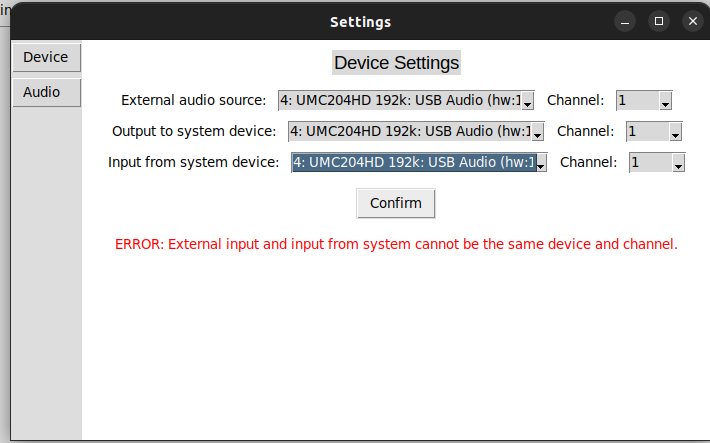
\includegraphics[width=0.8
	\linewidth]{Figures/DevSet.png}
	\caption{Device Settings page showing a red message because the user selected an invalid configuration.}
	\label{fig:Device Settings}
\end{figure}

\subsection{Audio Settings}

On this page, just like in the previous one, I will use a questionnaire-style interface with dropdown menus to define the Sample Rate, Bit Depth, and Block Size to be used.

For the Sample Rate and Bit Depth, I will suggest the most common values — such as 44,100 Hz, 48,000 Hz, 96,000 Hz, and 192,000 Hz for the sample rate, and 16, 24, and 32 bits for bit depth. However, the user is free to enter any value. The same applies to the Block Size.

At the bottom of the page, there is also a "Confirm" button, similar to the one in the "Device Settings" page. It performs basic checks, updates the selected values, and displays a message: green if everything is OK, orange in case of a warning (it applies the changes but alerts the user when a non-recommended or uncommon value is entered), and red if the Block Size is not a power of two — something required for the algorithms to work properly.

\begin{figure}[H]
	\centering
	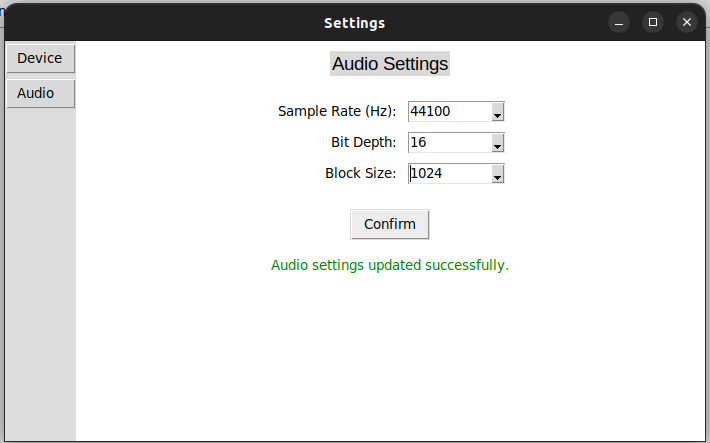
\includegraphics[width=0.8
	\linewidth]{Figures/AudSet.png}
	\caption{Audio Settings page showing a green message.}
	\label{fig:Audio Settings}
\end{figure}



\section{Acoustics analysis}

The acoustic analysis is devoloped with python librari LIBROSA\cite{librosa}

\subsection{Spectrogram (FT)}

How implemented the spectogram

\subsection{RTA [DONE]}

Usually, any form of analysis that is performed in real time can be considered \textbf{RTA} (\textit{Real-Time Analysis}). This includes a wide range of operations such as spectrum monitoring, transfer function measurements, phase and coherence analysis, and more—all happening as the signal flows. However, in my experience, in common usage, when someone refers to "RTA", they are often specifically referring to the classic 31-band graphical spectrum display. Also, the data collected on this page is especially important because it will be used to set the correction parameters. For all of that, this page has been named \textbf{RTA}.

Also, there is another conflict. When someone defines the 31 bands and their bandwidth, it is common to use the definition provided in \textbf{IEC 61260}. However, this standard does not mathematically respect the logarithmic spacing between bands. The 31 bands are defined as 1/3 of an octave per band.

\begin{table}[H]
\centering
\caption{Center frequencies for true 1/3 octave bands and IEC 61260 bands} 

	\scalebox{0.53}{
		\begin{tabular}{|c|c|c|c|c|c|c|c|c|c|c|c|}
			\hline
			1/3 octave & 19.69 & 24.8 & 31.25 & 39.37 & 49.61 & 62.5 & 78.75 & 99.21 & 125 & 157.49 & \\ \hline
			IEC 61260 & 20 & 25 & 31.5 & 40 & 50 & 63 & 80 & 100 & 125 & 160 & \\ \hline
			 & & & & & & & & & & & \\ \hline
			1/3 octave & 198,43 & 250 & 314.98 & 396.85 & 500 & 629.96 & 793.7 & 1000 & 1259.92 & 1587.4 & \\ \hline
			IEC 61260 & 200 & 250 & 315 & 400 & 500 & 630 & 800 & 1000 & 1250 & 1600 & \\ \hline
			 & & & & & & & & & & & \\ \hline
			1/3 octave & 2000 & 2519.84 & 3174.8 & 4000 & 5039.68 & 6349.6 & 8000 & 10079.37 & 12699.21 & 16000 & 20158.74 \\ \hline
			IEC 61260 & 2000 & 2500 & 3150 & 4000 & 5000 & 6300 & 8000 & 10000 & 12500 & 16000 & 20000 \\ \hline
				
		\end{tabular}
	}
\end{table}

\begin{minted}[label=\texttt{ipython}]{python3}
	"""
	In order to obtain the true 1/3 octave values, the following line of code was used with IPython3.
	The results were rounded to the second decimal place.
	"""
	
	[round(1000*2**(band/3), 2) for band in range (-17,14)]
	
\end{minted}

On the other hand, this standard is widely used in many professional devices and software. One important example is the DBX 231s graphic equalizer, which is commonly used in analog processing chains.

\begin{figure}[H]
	\centering
	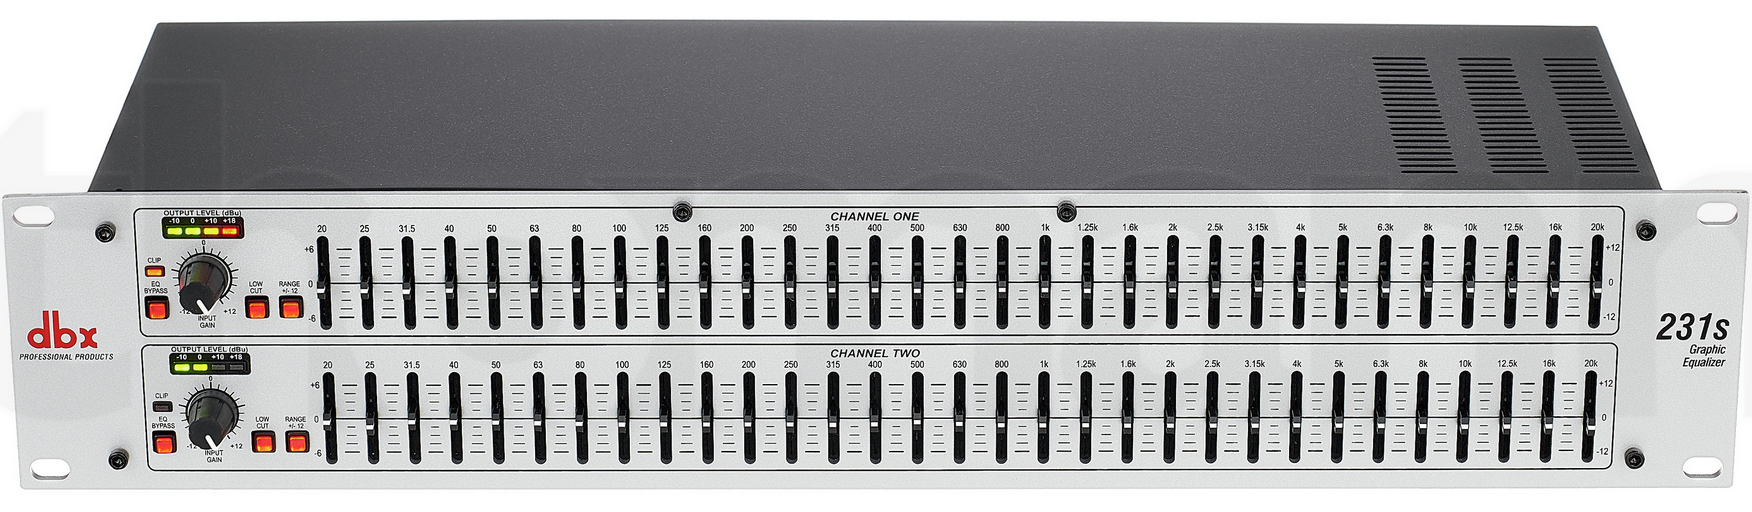
\includegraphics[width=1
	\linewidth]{Figures/DBX_231s.png}
	\caption{Image of the front panel of the DBX 231s \cite{DBX_31s}, where we can observe that the center frequency bands are the same as those defined in IEC 61260.}
	\label{fig:DBX_31s}
\end{figure}

In order to achieve the greatest possible compatibility and coherence with industry standards, I prefer to use the IEC 61260 standard.


The signal path on this page is very similar to the one used on the "FT" page. We have a buffer with two blocks of input data ("Input from external device" and "Input from system").

First, we copy the buffer data to the "delay buffer", where, if needed, the data will be adjusted to make it coincide with the applied delay. If necessary, the adjustment will use data from previous blocks stored in the same "delay buffer".

I created this buffer with the capacity to store 1 second of data, which can be used to apply a maximum delay of (1 - "Block Size in seconds") seconds.

Once the data in the "delay buffer" is adjusted, we can start applying algorithms to perform the analysis.

The algorithm is based on the calculation of RMS (\textit{root mean square}) to obtain the energy for each frequency band, which is divided using filters for each band.


\begin{figure}[H]
	\begin{center}
		\vspace{-2mm}
		\tikzsetnextfilename{RTA_page_schem}
		\begin{tikzpicture}[node distance=30mm,on grid,auto, scale=1, bend angle=45]
			
			every node/.style={font=\small};
			
			\node (q_init) [draw, rectangle, minimum size=1cm,] {Input Buffer};
			\node (null_init) [right=of q_init] {};
			\node (q_delay) [draw, rectangle, minimum size=1cm, right=of null_init] {Delay Buffer};
			\node (q_ext) [draw, rectangle, minimum size=1cm, above right=of q_delay, xshift=2cm] {Filtering and RMS Calculation of External Input};
			\node (q_in_sys) [draw, rectangle, minimum size=1cm, below right=of q_delay, xshift=2cm] {Filtering and RMS Calculation of Input from System};
			\node (q_diff) [draw, rectangle, minimum size=1cm, right=of q_delay, xshift=4cm] {Difference calculation};	
			
			\draw[blue, very thick, ->] (q_init) edge node {2 channels} (q_delay);
			\draw[blue, dotted, very thick, ->] (q_delay) edge[bend right=10] node {1 channel} (q_ext);
			\draw[blue, dotted, very thick, ->] (q_delay) edge[bend right=10] node {1 channel} (q_in_sys);
			\draw[green, very thick, ->] (q_ext) edge[bend right=10] node {Analysis Data} (q_diff);
			\draw[green, very thick, ->] (q_in_sys) edge[bend right=10] node {Analysis Data} (q_diff);
			
		\end{tikzpicture}
		\vspace{-2mm}
	\end{center}
	\caption{Diagram of the architecture of the RTA page}
\end{figure}


In this case, I'm not using any kind of windowing. As a starting point, I'm using 4th-order IIR (\textit{infinite impulse response}) Butterworth band-pass filters for each band. All these filters are created using the \texttt{scipy.signal} library \cite{scipy_signal}, which returns SOS (\textit{Second-Order Section}) parameters.

\begin{figure}[H]
	\centering
	\caption{Second-Order Sections for IIR filters with their parameters}
	\[
	H(z) = \frac{b_0 + b_1 z^{-1} + b_2 z^{-2}}{1 + a_1 z^{-1} + a_2 z^{-2}}
	\]
\end{figure}

When the program applies each filter to the signal block, it also calculates the RMS and converts it to a logarithmic scale, which will be plotted on the graph and used to calculate the difference graph.

\begin{figure}[H]
	\centering
	\caption{Root Mean Square to calculate energy from filtered signal}
	\[
	RMS = \sqrt{ \frac{1}{N} \sum_{n=0}^{N-1} x^2[n] }
	\]
\end{figure}

At the end, there is: a pause button, which blocks the update function and can be used to pause the graphics; a save button, to store the current values of the difference graph for later use in the correction window; and a time averaging section that works exactly the same as the averaging section from the FT page, except that it does not include frequency averaging (since it doesn't make sense to apply frequency averaging between bands).

\begin{figure}[H]
	\centering
	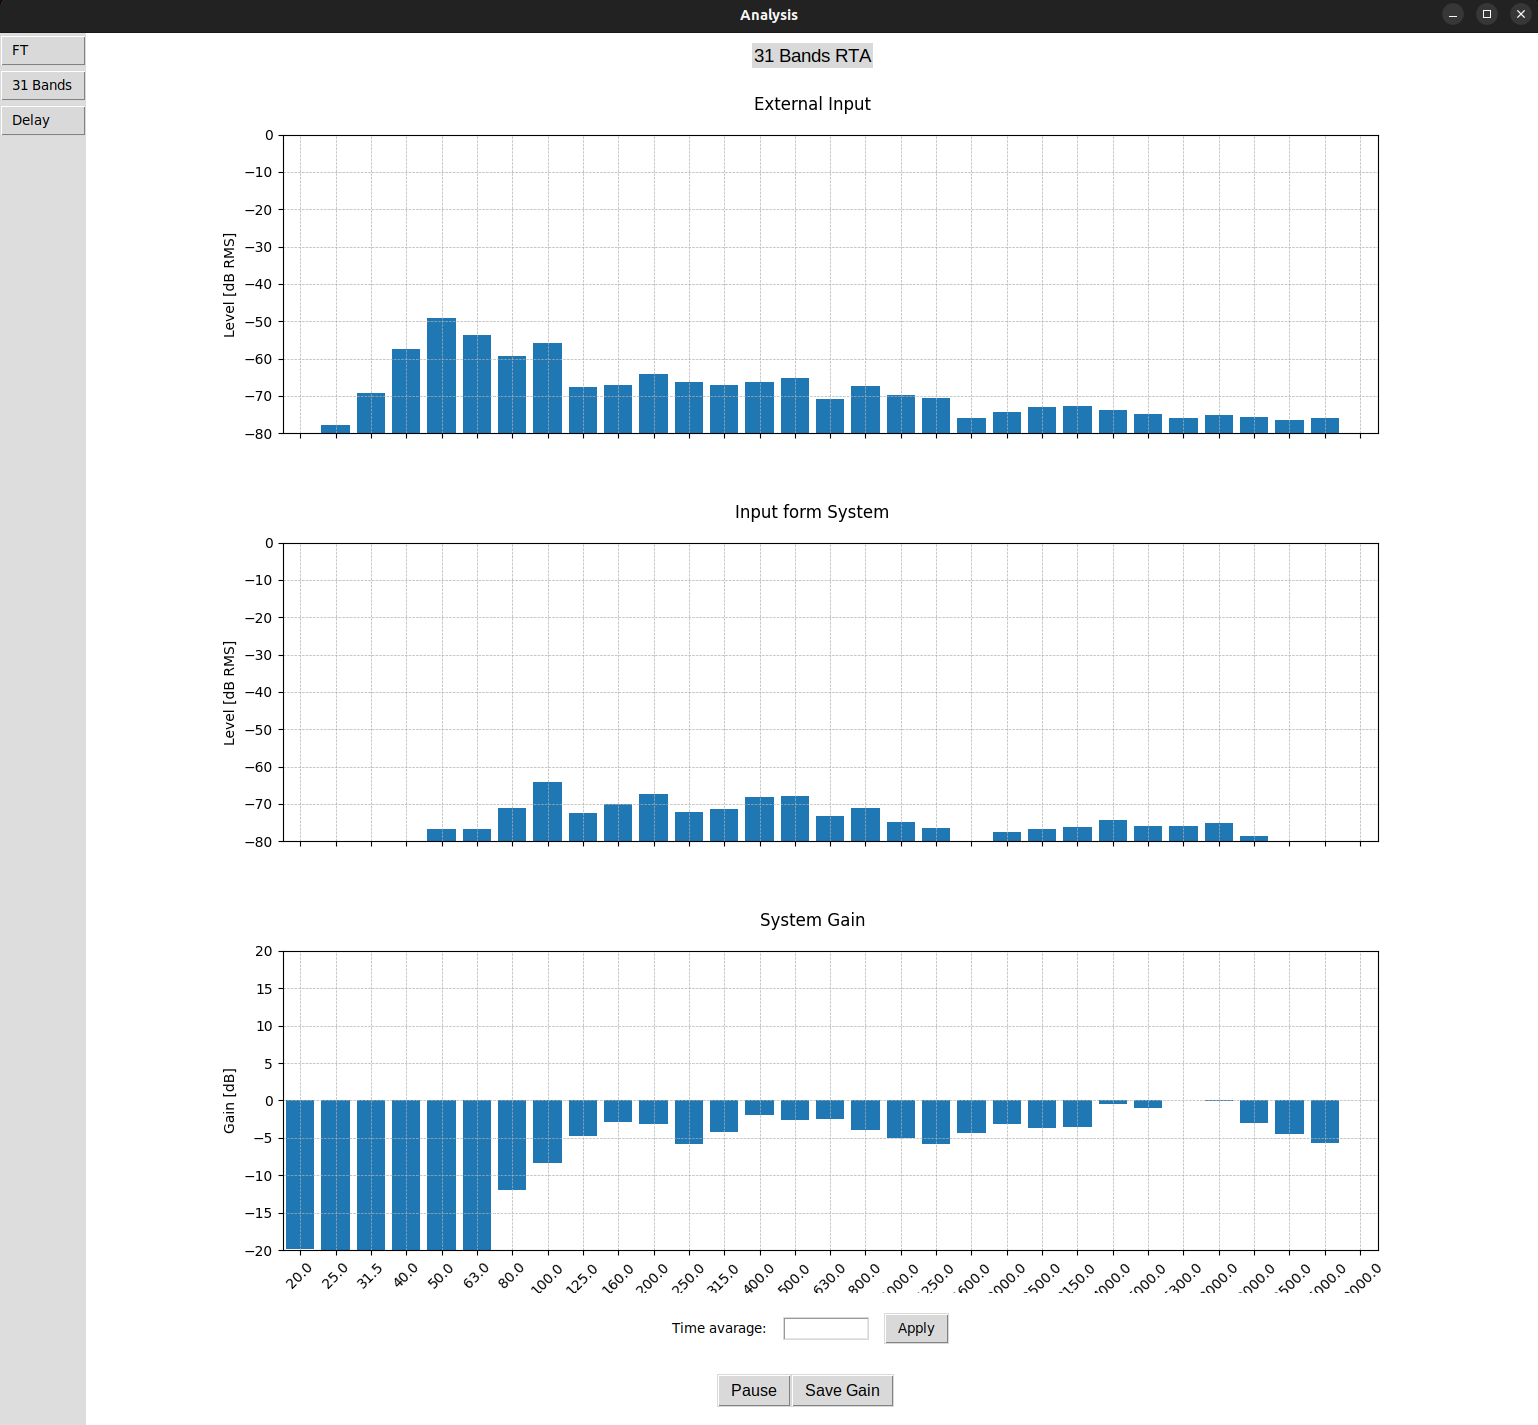
\includegraphics[width=1
	\linewidth]{Figures/RTA_page.png}
	\caption{Analysis window - RTA page.}
	\label{fig:DBX_31s}
\end{figure}


\subsection{Delay}

Explain delay page

\section{Acoustic correction}

Acoustic correction = DSP, allways have to be somethuing on the output buffer, by default, zeros.

\subsection{Bypass}

How Bypass works, and why it works bad.

\subsection{31 Bars}

Implementation of correction

\section{Integration of monitoring mechanism}

Home page and information that it appears / start, stop streams buttons...

\section{Others}

More problems that I didn't expect, losing time solving them or at least trying to. No more time to implement additional functionalities...